%% ------------------------------------------------------------------------- %%
\chapter{Resultados}
\label{cap:resultados}

%% ------------------------------------------------------------------------- %%
%% ------------------------------------------------------------------------- %%
\section{Experimentos}
  Os objetivos dos experimentos são: (i) comparar o impacto de cada umas das
melhorias de desempenho apresentadas na seção \ref{melhoriaDesempenho} aplicadas
individualmente; (ii) estudar a correlação entre duas melhorias aplicadas ao
mesmo tempo; (iii) tentar identificar métricas para decidir em qual ambiente
cada passo deve ser executado, baseando-se nas entradas do registro.

  As melhorias de desempenho podem ser ativadas independentemente nos testes,
controladas atráves de um arquivo de configuração, passado como entrada para os
testes. Logo, usando os mesmos dados, os seguintes testes são executados:

\begin{enumerate}
  \item Paralelamente em CPU (nosso \textit{guideline})
  \item GPU sem nenhuma das melhorias ativadas
  \item GPU com a interpolação executando em CPU
  \item Melhoria de cálculo de Ocupação
  \item Melhoria de textura 3D
  \item Melhoria de execução em paralelo
  \item Todas as combinações de duas melhorias ativas por vez
  \item Todas as melhorias ativas
\end{enumerate}

  Os testes consistem de quatro registros, sempre da mesma imagem alvo para a
mesma imagem referência, com cada uma das quatro execuções utilizando um
conjunto cada vez maior de caracteristicas. Como visto na seção
\ref{thinPlateSplines}, o tempo de execução do algoritmo cresce com o cubo do
número de características, e o número de threads necessárias para executar o
kernel cresce com o tamanho da imagem, logo aumentar o número de características
é a melhor escolha para aumentar a complexidade das instâncias diferentes de
registro.

  A imagem referência foi adiquirida no software \cite{papademetris2005bioimage}.
A imagem alvo foi criada aplicando uma deformação senoidal nas três dimensões da
imagem referência, ver figura \ref{fig:testImg}. A construção artificial das
imagens alvo foi realizada pelos seguintes motivos: (1) provar a aplicabilidade
do algoritmo TPS não é nosso objetivo, (2) com a função que provocou a
deformação em mãos, gerar um conjunto de características se torna um processo
trivial, assim como encontrar as correspondências entre elas, e (3) a corretude
da nossa implementação do TPS é facilmente verificavel. A função de deformação
escolhida foi:

\begin{align} \label{math:composta}
\begin{split}
  X &= x + 2*sin(\frac{y}{8}) - 2*cos(\frac{z}{16}) \\
  Y &= y + 4*sin(\frac{x}{8}) - 2*sin(\frac{z}{8}) \\
  Z &= z + 2*sin(\frac{x}{16}) - 4*cos(\frac{y}{8})
\end{split}
\end{align}

  Os coeficientes utilizados na função acima foram escolhidos para criar uma
deformação que não seja muito intensa, onde mesmo com um mapeamento trivial
entre as características o TPS não seria capaz de registrar as imagens, mas
intensa o suficiente para deslocar pontos da imagem para longe de sua região
inicial, o que fará com que threads responsáveis pelo seu registro tenham que
acessar regiões diferentes na memória da GPU, criando uma situação menos
favorável para a implementação do registro em CUDA e mais próxima do real.

\begin{figure}[H]
    \centering
    \begin{subfigure}[t]{0.8\textwidth}
      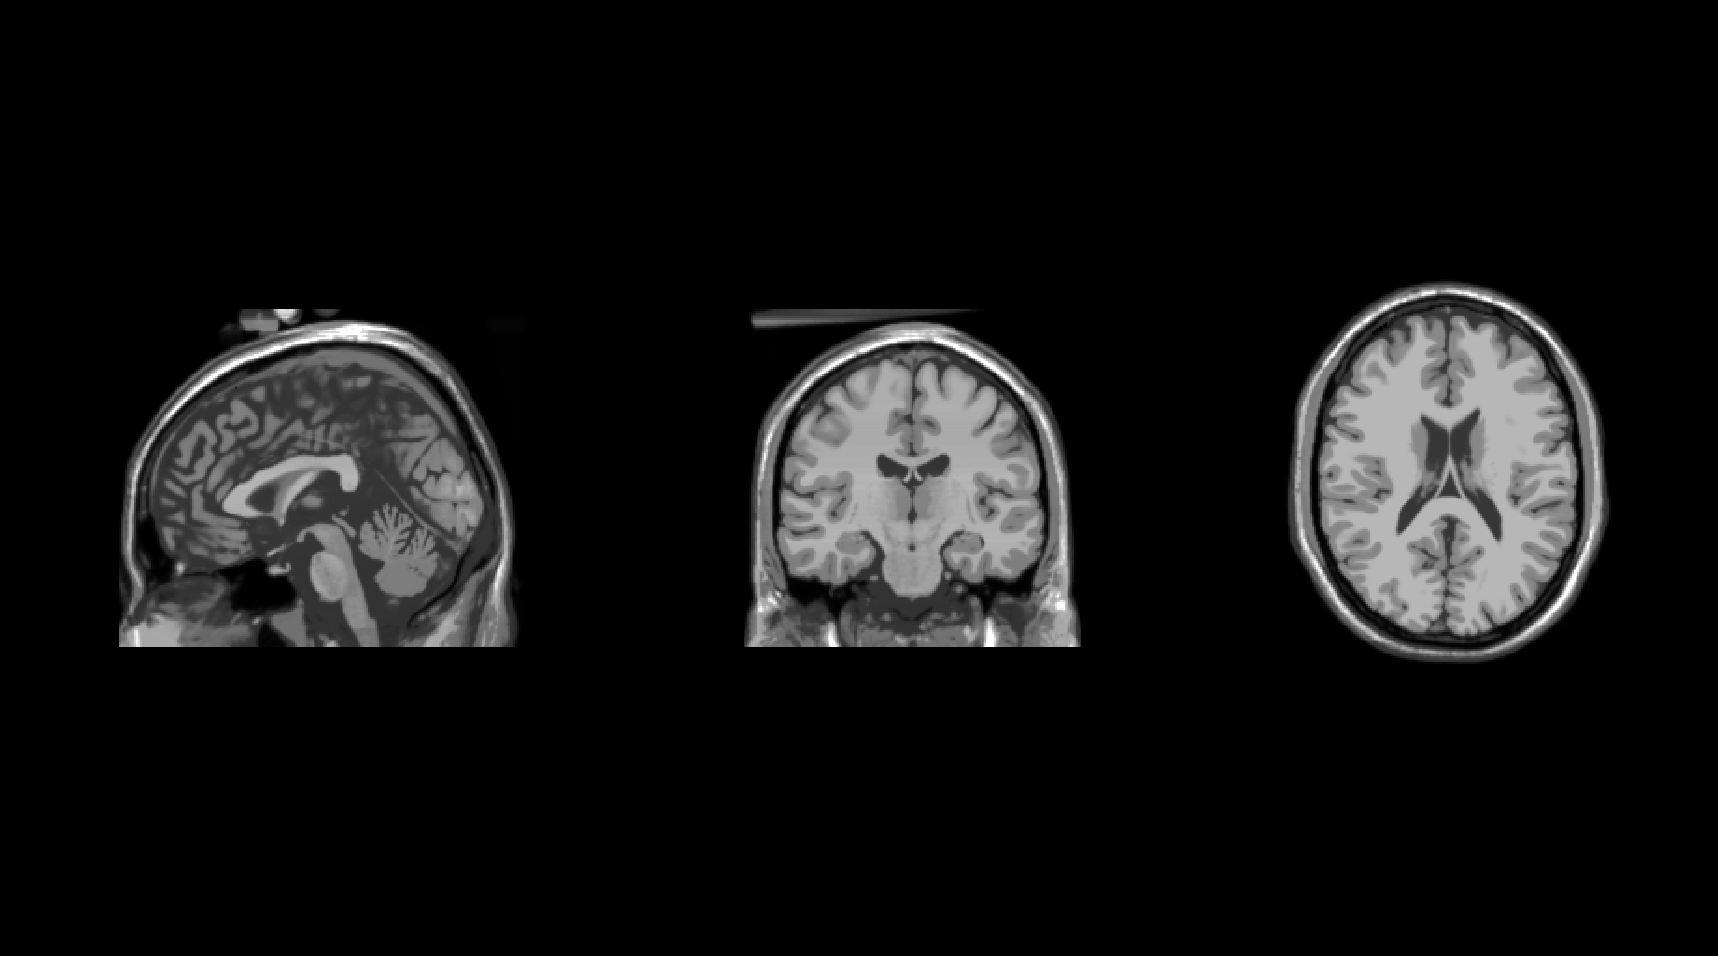
\includegraphics[width=\textwidth]{figuras/referenceImg.png}
      \subcaption*{(a)}
      \label{fig:refImg}
    \end{subfigure}
    \begin{subfigure}[t]{0.8\textwidth}
      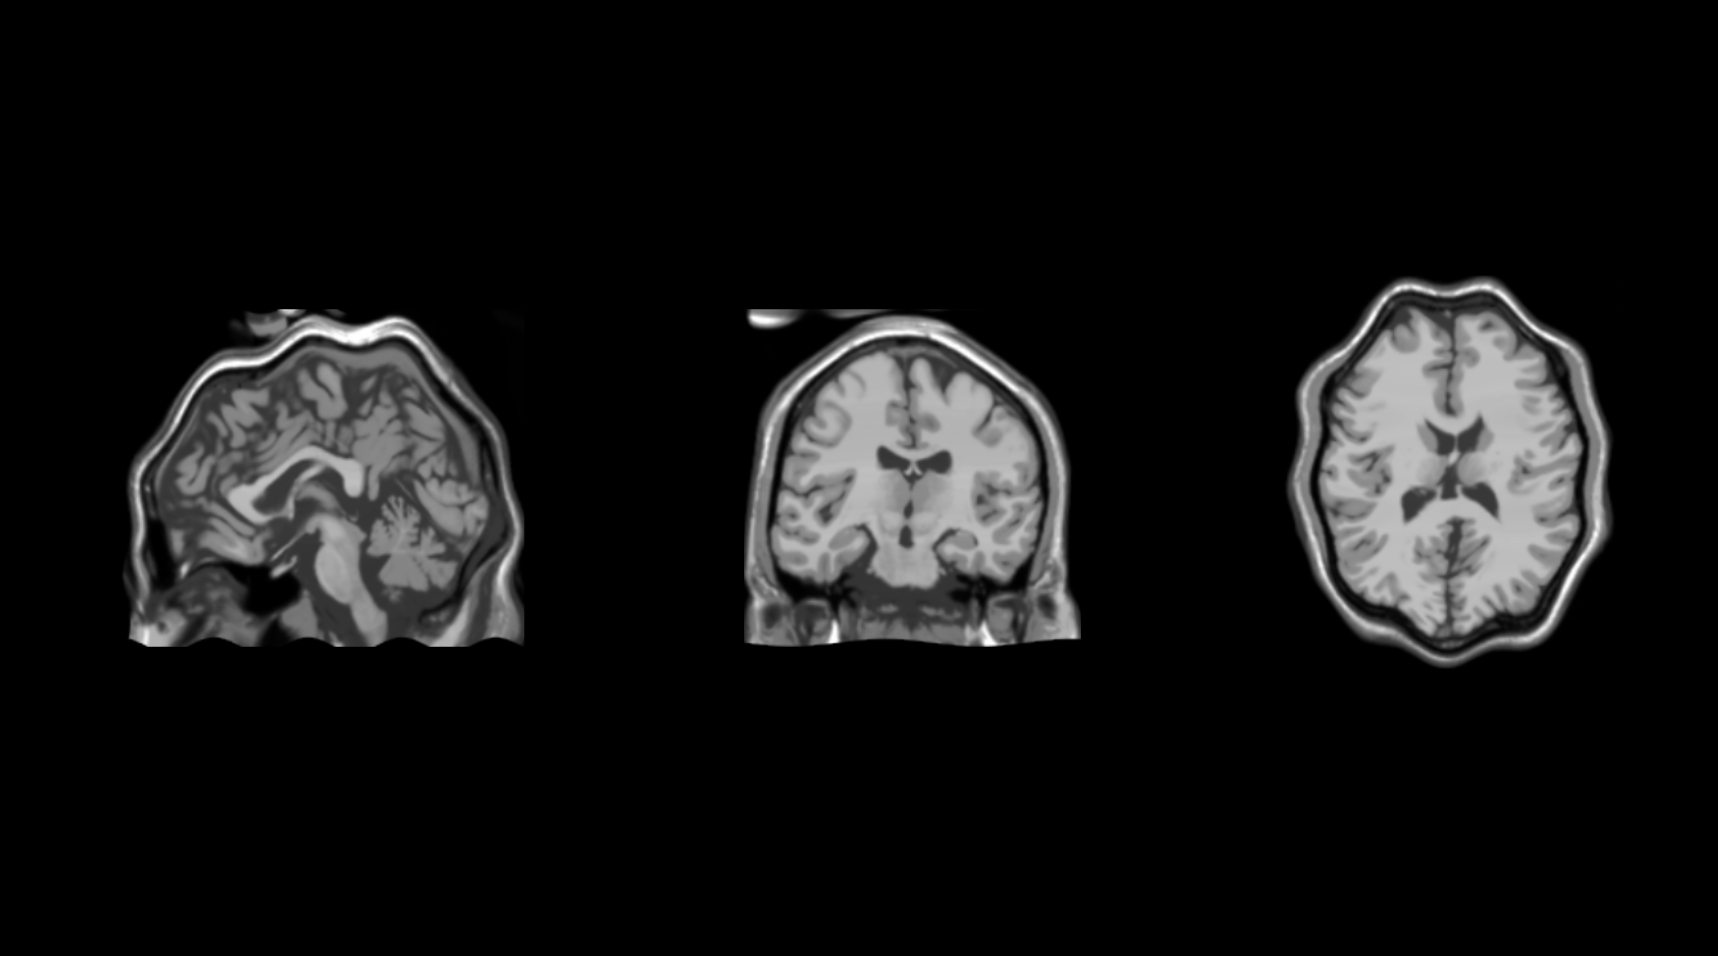
\includegraphics[width=\textwidth]{figuras/targetImg.png}
      \subcaption*{(b)}
      \label{fig:tarImg}
    \end{subfigure}
    \source{\cite{papademetris2005bioimage}}
    \caption{Imagens usadas nos testes. A primeira coluna é um corte sagital,
             a segunda coluna um corte coronal e a última um corte axial.
             (a) Imagem referência. (b) Imagem alvo.}
    \label{fig:testImg}
\end{figure}

  As características da imagem referência são distribuidas uniformemente pelas
dimensões da imagem, com um fator que determina a quantidade de características
utilizadas. As características da imagem alvo são construidas aplicando a
função de deformação em cada uma das características da imagem referência,
criando um cenário ideal para a execução do TPS, onde sabemos o mapeamento de
cada uma das características da imagem referência.

  Os testes foram executados em duas máquinas. A primeira é um notebook com
um processador quadcore Intel i5-3337U @ 1.80GHZ, 6GB de memória, e uma GPU
NVIDIA GeForce GT 730M com 384 cuda cores divididos em 2 multiprocessadores e
2GB de memória dedicada. A segunda máquina é uma máquina virtual, com 4
processadores de 2.3GHz, 8GB de memória, e uma GPU GeForce GTX 980 com 2048
cuda cores divididos em 16 multiprocessadores e 4GB de memória dedicada.

\begin{figure}[H]
    \centering
    \begin{subfigure}[t]{0.5\textwidth}
      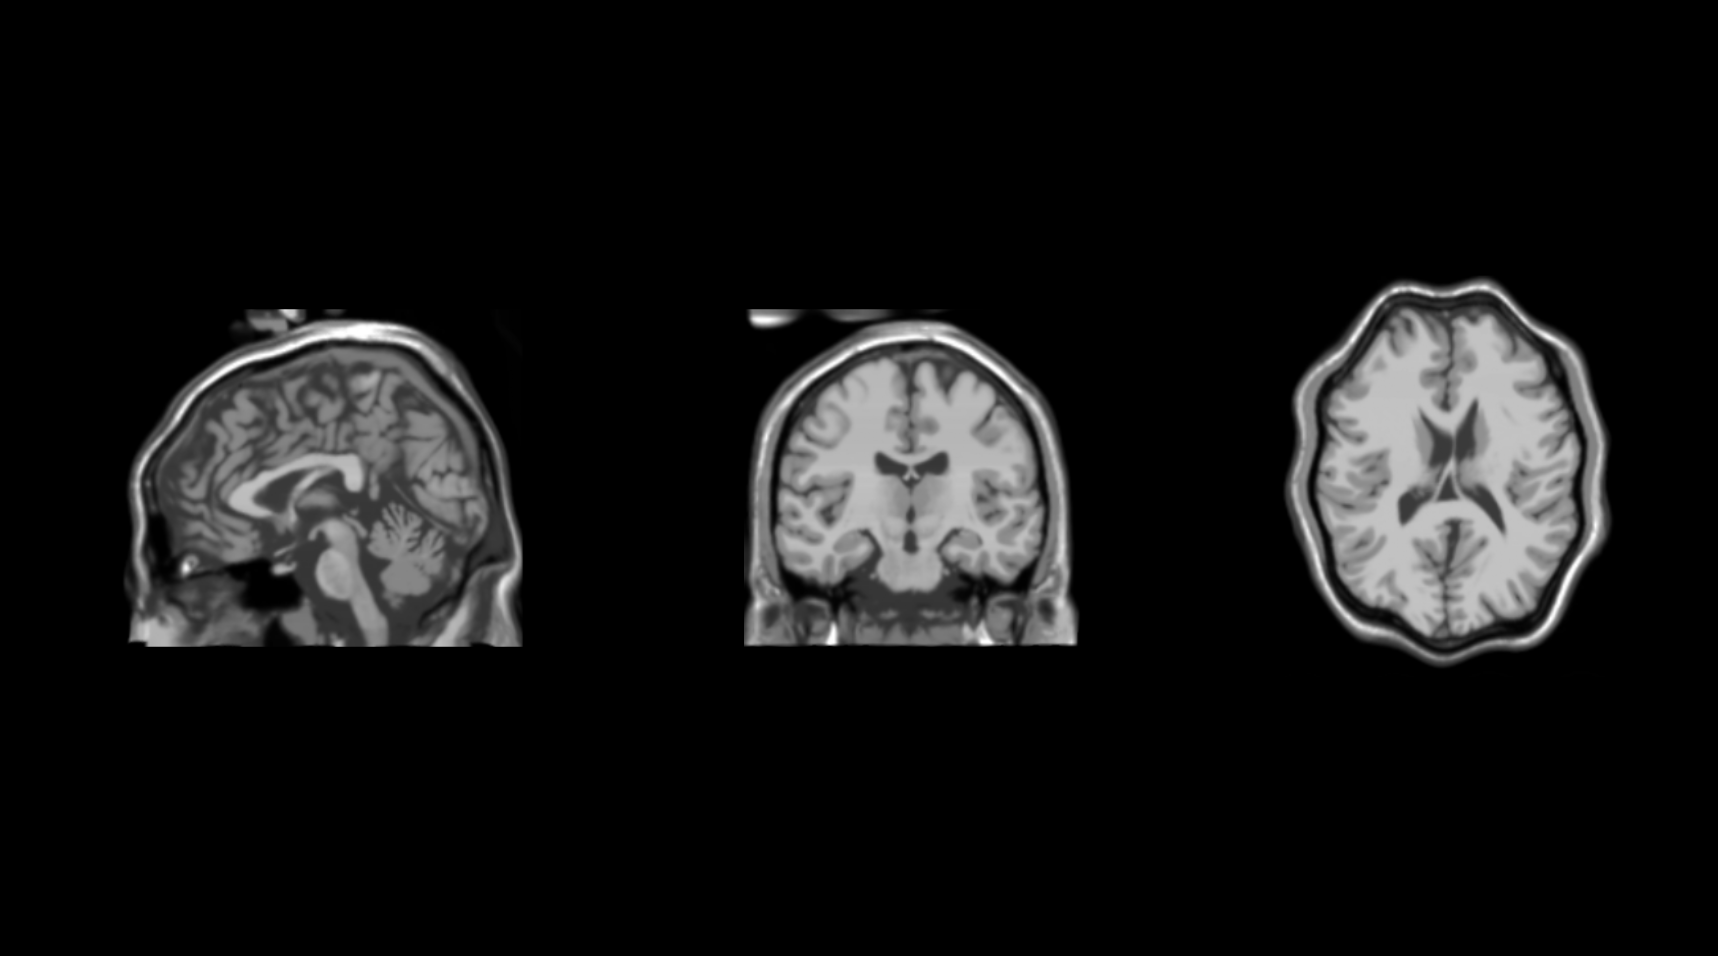
\includegraphics[width=\textwidth]{figuras/result001.png}
      \subcaption*{(a)}
      \label{fig:unequalizedImage}
    \end{subfigure}
    \begin{subfigure}[t]{0.5\textwidth}
      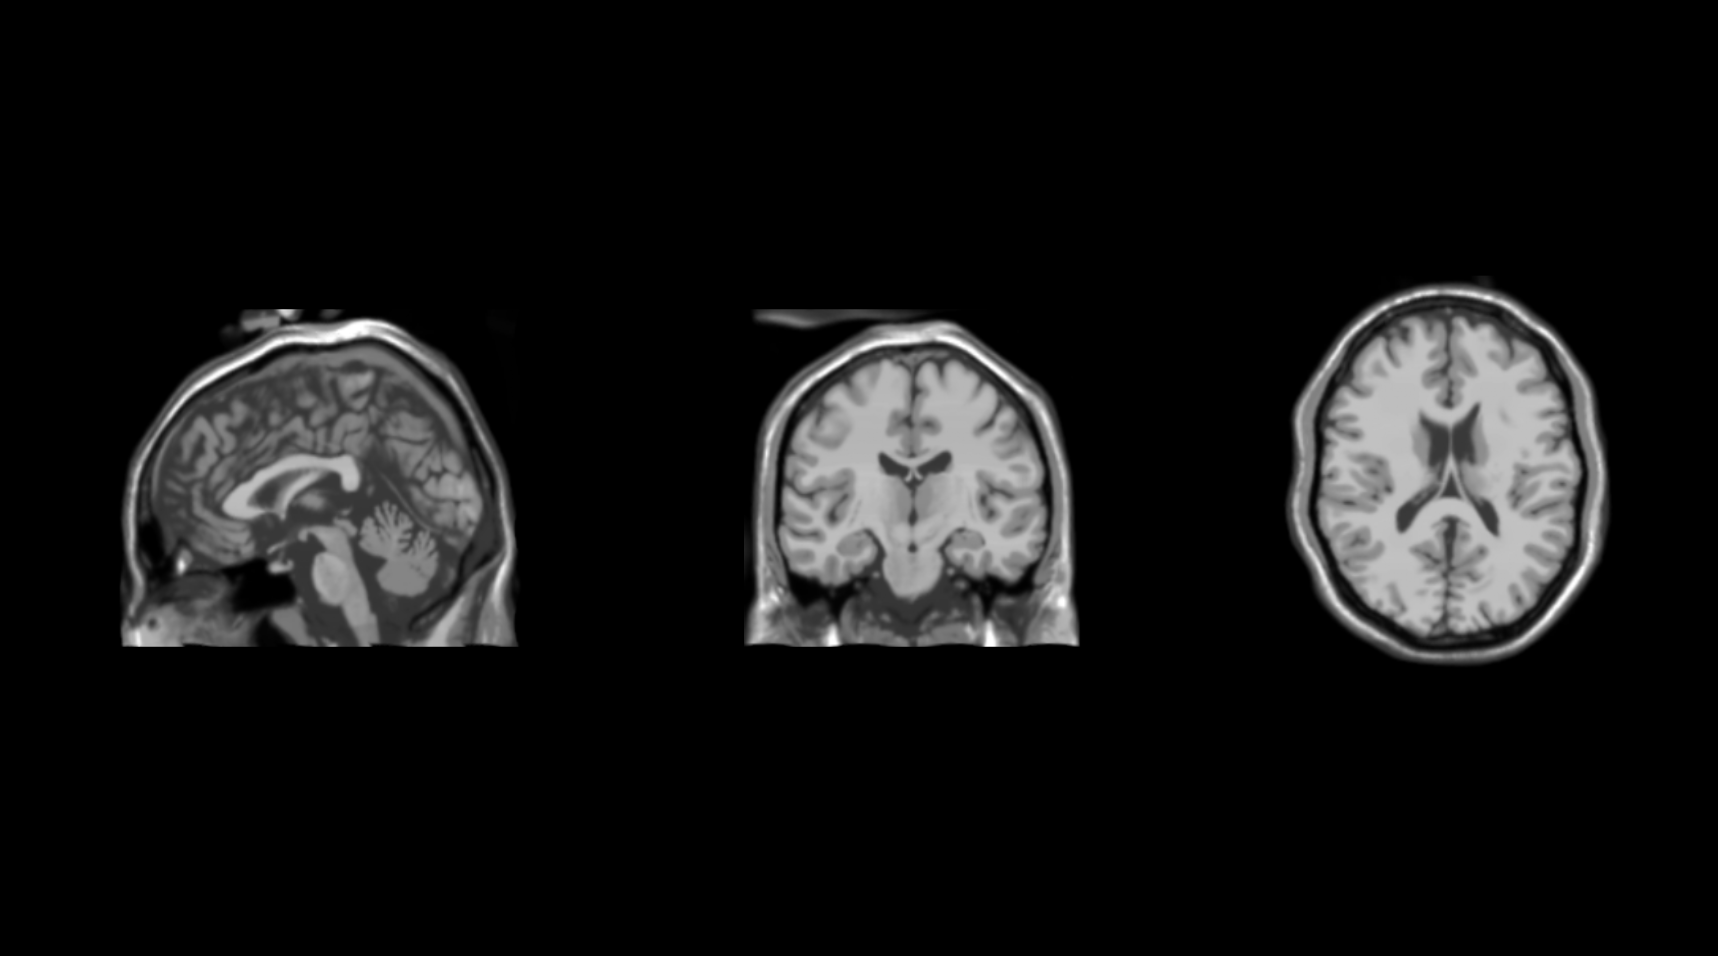
\includegraphics[width=\textwidth]{figuras/result002.png}
      \subcaption*{(b)}
      \label{fig:equalizedImage}
    \end{subfigure}
    \begin{subfigure}[t]{0.5\textwidth}
      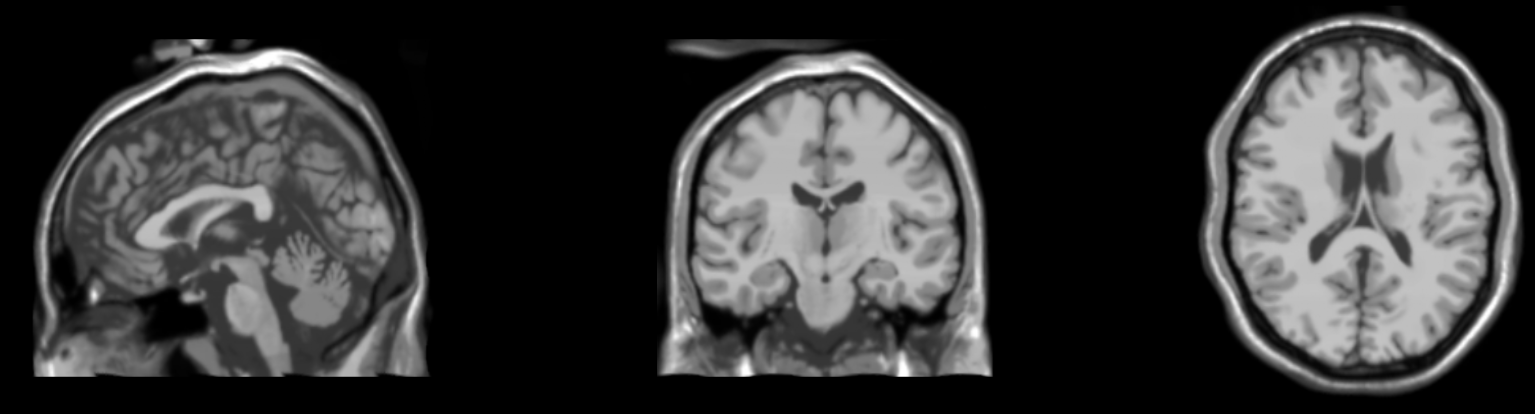
\includegraphics[width=\textwidth]{figuras/result003.png}
      \subcaption*{(c)}
      \label{fig:equalizedImage}
    \end{subfigure}
    \begin{subfigure}[t]{0.5\textwidth}
      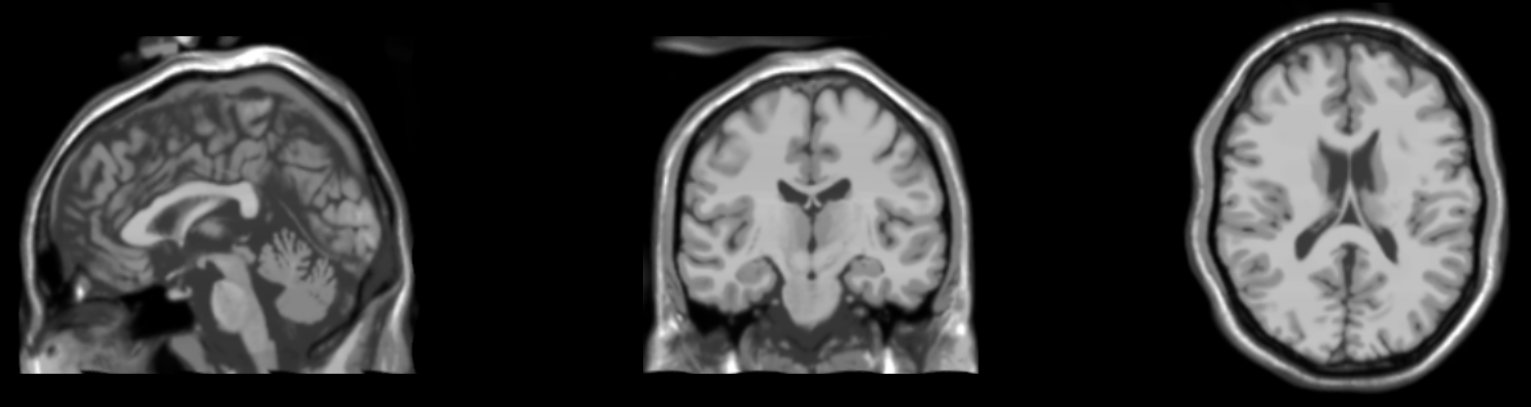
\includegraphics[width=\textwidth]{figuras/result004.png}
      \subcaption*{(d)}
      \label{fig:equalizedImage}
    \end{subfigure}
    \caption{Resultado dos testes. A primeira coluna é um corte sagital,
             a segunda coluna um corte coronal e a última um corte axial.
             (a) Resultado utilizando 576 características.
             (b) Resultado utilizando 2016 características.
             (c) Resultado utilizando 4864 características.
             (d) Resultado utilizando 7942 características.}
    \label{fig:equalization}
\end{figure}
